\documentclass[9pt, twocolumn]{article}
\usepackage{pgfplots}
\usepackage{layout}
\usepackage{graphicx}
\usepackage{amsmath}
\usepackage{caption}
\usepackage{subfig}
\usepackage{adjustbox}
\usepackage[left=2cm,right=2cm,top=2cm,bottom=2cm]{geometry}
\graphicspath{G:/Shared drives/ME_FIA_Spruce/ME_FIA_Spruce/doc}

%opening
\begin{document}
	\title{High Resolution Estimates of Spruce-Site-Suitability in Maine}
	\author{Ashley Carter and Mike Premer \\
		Maine Forest Management Laboratory\\}

\maketitle
\section{Introduction}
Precision silvicultural applications require baseline estimates of site productivity and species-specific factors that may limit occurrence or influence growth. In Maine, native spruce species (red spruce-Picea rubens, white spruce-Picea glauca, and black spruce-Picea mariana) are commonly managed for commodity production, wildlife habitat, and non-timber income. Yet, each species requires specific environmental settings that parallel silvics and functional traits for survival and optimal growth. While it is acknowledged that matching Picea spp. with site-specific growing conditions may effectively increase survival and realized productivity, little work has been conducted at a resolution compatible with management activities (i.e., within-stand). The goal of this project was to integrate climate data, remote sensing products, and publicly available field data to develop high-resolution predictive mapping systems of species-site-suitability for native spruce species across Maine. 
\section{Methods}
A total of 10,423 plot measurements were obtained at the tree, sapling, and seedling level from the United States Forest Service Forest (USFS) Forest Inventory and Analysis Program (FIA), the Maine Natural Areas Program (MNAP), and the National Aeronautics and Space Administration (NASA) Carbon Monitoring System (CMS) program (Figure 1). Climate data, digital soil maps, and topographic covariates were used to estimate site-specific trends for each species of interest and selected with the decision-tree based VSURF procedure, and tested with a mixed-effects logistic regression model with the standard approach: 
\begin{multline}
	\operatorname{Pr}(\text{Spruce} = 1)\\
	= \frac{\exp(\beta_{0} + \beta_{1} \text{STAND} + \beta_{2} \text{SITE} \dots +\beta_{3} \text{CLIM)} }{1 + \exp(\beta_{0} + \beta_{1} \text{STAND} + \beta_{2} \text{SITE} \dots +\beta_{3 }\text{CLIM})}
\end{multline}
\setlength\parindent{0pt}
where p(s=1) is the probability of the ith spruce species occurring, and STAND, SITE, and CLIM correspond to stand metrics (e.g., basal area), site conditions (e.g., elevation, aspect) and climate attributes (e.g., mean temperature, precipitation), respectively. Spatial autocorrelation was estimated through a semi-variogram procedure. Candidate models were compared through AUC scores, and final models were standardized to provide a relative index of species suitability (Suitability Index = observed(p)/max(p)). 
Final models were used to generate statewide estimates of suitability at the common resolution of 1/5 acre throughout Maine. Estimates of uncertainty were generated through a Kriging spatial interpolation process of model residuals. 
\section{Results and Discussion}
Results highlight a strong pattern of black and white spruce with local hydrologic catchment area and evapotranspiration rates, respectively, while red spruce appeared to be relatively plastic in comparison (i.e., did not exhibit sensitivity to local site conditions). All species exhibited trends with climatic variables, including vapor pressure deficit, mean precipitation, and maximum temperature (Table 1). AUC scores ranged from 0.94 (red spruce), 0.96 for white spruce, and 0.99 for black spruce, indicating high level of model performance. Across Maine, the range in relative suitability follows general trends in elevation and climate patterns (Fig 1a), which can be downscaled to user-specific domains, as demonstrated with currently delineated stand boundaries (Fig 1b). These tools can be used to [1] Tailor harvest prescriptions and ensure the most appropriate species are the focus of silviculture; [2] Identify priority areas for artificial regeneration and planted forests; [3] Guide timber stand improvement activities, including density management regimes: [4] Serve as a framework to support forest habitat classification; and [5] Calibrate growth and yield models. Geospatial data can be sourced at https://www.maineforestlab.com/single-project
\section{Acknowledgments}
The Maine Agricultural and Forest Experiment Station (MAFES) provided project funding and student support.  

\onecolumn

\begin{figure}%
	\centering
	\subfloat[\centering]{{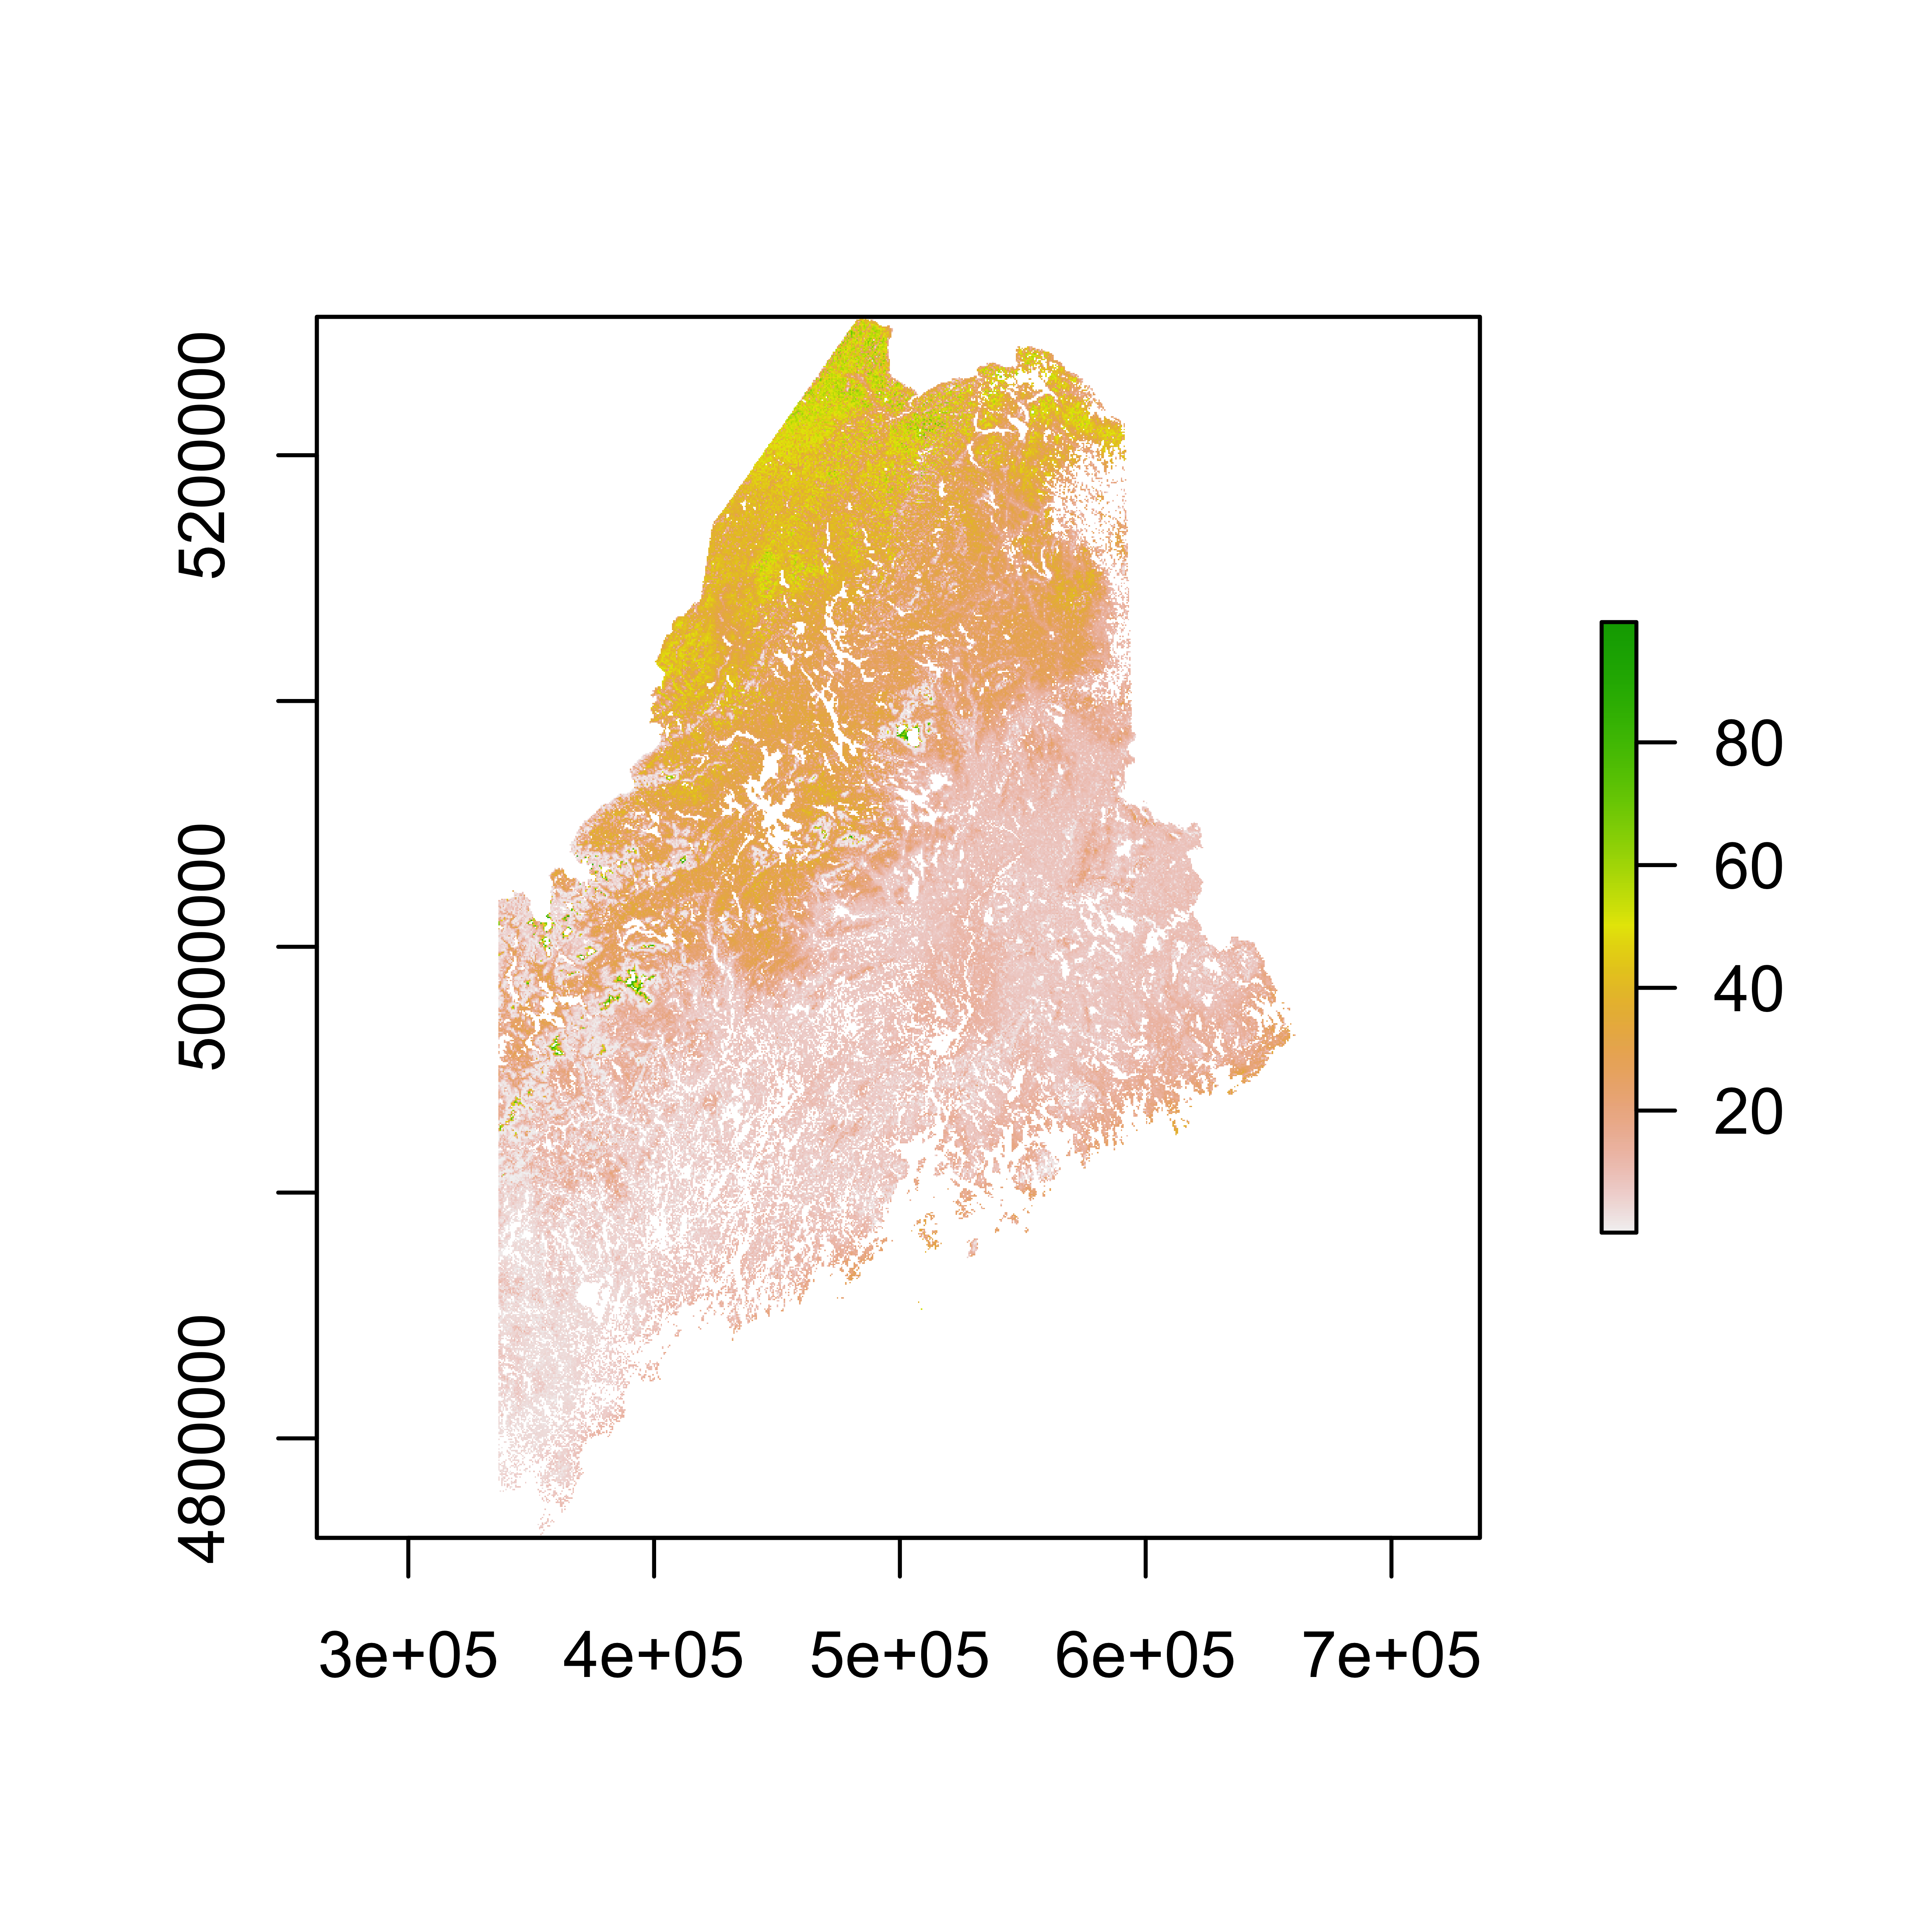
\includegraphics[width=8.25cm]{WS_Suit_demo_StateWide2.png} }}%
	\qquad
	\subfloat[\centering]{{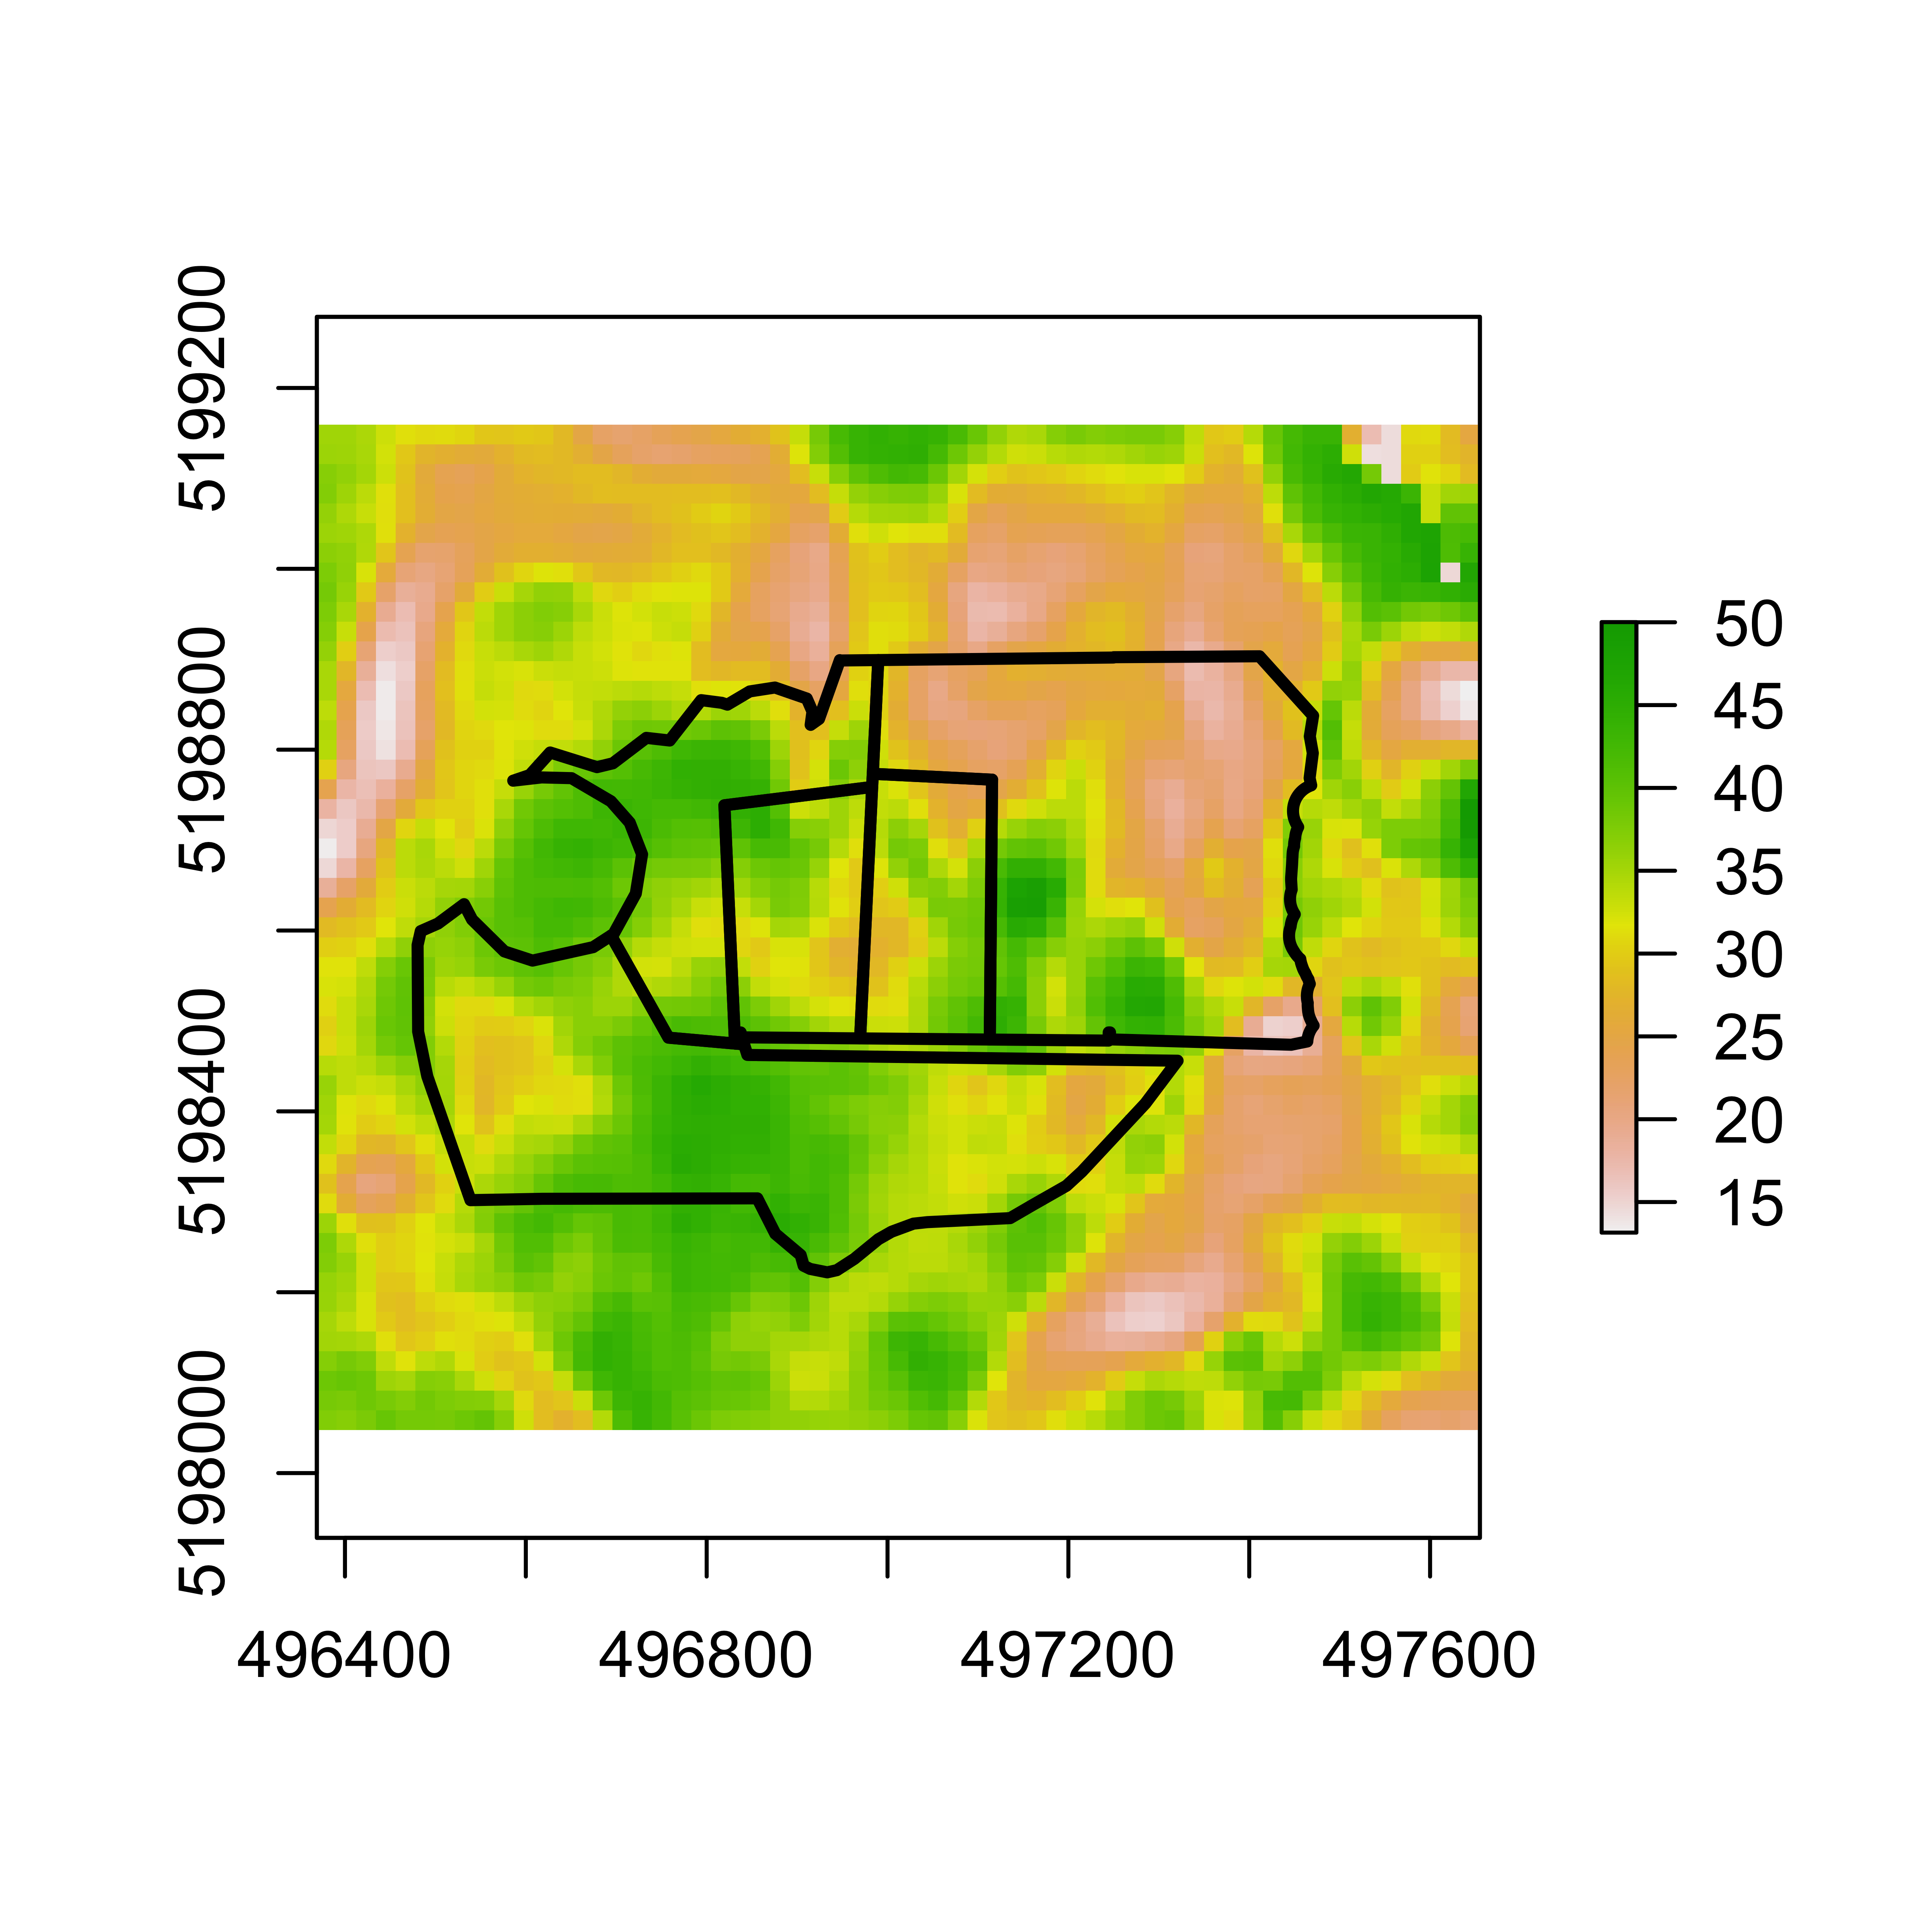
\includegraphics[width=8.25cm]{WS_Suit_demo.png} }}%
	\caption{Statewide estimates of contemporary WS site suitability (0-100) across Maine (left panel -a) and downscaled to a designated planting block and stands (right panel-b). }%
	\label{fig:example}%
\end{figure}
\break
\break
\break
\break
\break
\break
\break
\break
\break
\begin{center}
	\captionof{table}{Species specific transformed odds ratios of site suitability given corresponding predictive variables, following equation 1. VPDMax, PPT, and Tmax are 3—year average vapor pressure deficit, precipitation, and maximum temperature, respectively, while TWI indicates topographic wetness index, and WSI is the water surplus index.
	\break}
	\begin{tabular}{|c c c c|} 
		\hline
		Parameter & BS & RS & WS \\ [0.5ex] 
		\hline\hline
		$\beta_{0}$ & 3.88 & 43.41 & 26.94 \\ 
		$\beta_{1}$\text{VPDmax} & 0.53 & 0.82 & - \\
		$\beta_{2}$\text{PPT} & 0.99 & - & - \\
		$\beta_{3}$\text{Tmax} & - & 0.80 & 0.71 \\
		$\beta_{4}$\text{TWI} & 2.47 & - &  \\
		$\beta_{5}$\text{WSI} & - & - & 0.99 \\ [1ex] 
		\hline
	\end{tabular}
\end{center}



\end{document}
